% Options for packages loaded elsewhere
\PassOptionsToPackage{unicode}{hyperref}
\PassOptionsToPackage{hyphens}{url}
%
\documentclass[
]{article}
\usepackage{lmodern}
\usepackage{amssymb,amsmath}
\usepackage{ifxetex,ifluatex}
\ifnum 0\ifxetex 1\fi\ifluatex 1\fi=0 % if pdftex
  \usepackage[T1]{fontenc}
  \usepackage[utf8]{inputenc}
  \usepackage{textcomp} % provide euro and other symbols
\else % if luatex or xetex
  \usepackage{unicode-math}
  \defaultfontfeatures{Scale=MatchLowercase}
  \defaultfontfeatures[\rmfamily]{Ligatures=TeX,Scale=1}
\fi
% Use upquote if available, for straight quotes in verbatim environments
\IfFileExists{upquote.sty}{\usepackage{upquote}}{}
\IfFileExists{microtype.sty}{% use microtype if available
  \usepackage[]{microtype}
  \UseMicrotypeSet[protrusion]{basicmath} % disable protrusion for tt fonts
}{}
\makeatletter
\@ifundefined{KOMAClassName}{% if non-KOMA class
  \IfFileExists{parskip.sty}{%
    \usepackage{parskip}
  }{% else
    \setlength{\parindent}{0pt}
    \setlength{\parskip}{6pt plus 2pt minus 1pt}}
}{% if KOMA class
  \KOMAoptions{parskip=half}}
\makeatother
\usepackage{xcolor}
\IfFileExists{xurl.sty}{\usepackage{xurl}}{} % add URL line breaks if available
\IfFileExists{bookmark.sty}{\usepackage{bookmark}}{\usepackage{hyperref}}
\hypersetup{
  pdftitle={Remote Sensing in the Social Sciences},
  hidelinks,
  pdfcreator={LaTeX via pandoc}}
\urlstyle{same} % disable monospaced font for URLs
\usepackage[margin=1in]{geometry}
\usepackage{color}
\usepackage{fancyvrb}
\newcommand{\VerbBar}{|}
\newcommand{\VERB}{\Verb[commandchars=\\\{\}]}
\DefineVerbatimEnvironment{Highlighting}{Verbatim}{commandchars=\\\{\}}
% Add ',fontsize=\small' for more characters per line
\usepackage{framed}
\definecolor{shadecolor}{RGB}{248,248,248}
\newenvironment{Shaded}{\begin{snugshade}}{\end{snugshade}}
\newcommand{\AlertTok}[1]{\textcolor[rgb]{0.94,0.16,0.16}{#1}}
\newcommand{\AnnotationTok}[1]{\textcolor[rgb]{0.56,0.35,0.01}{\textbf{\textit{#1}}}}
\newcommand{\AttributeTok}[1]{\textcolor[rgb]{0.77,0.63,0.00}{#1}}
\newcommand{\BaseNTok}[1]{\textcolor[rgb]{0.00,0.00,0.81}{#1}}
\newcommand{\BuiltInTok}[1]{#1}
\newcommand{\CharTok}[1]{\textcolor[rgb]{0.31,0.60,0.02}{#1}}
\newcommand{\CommentTok}[1]{\textcolor[rgb]{0.56,0.35,0.01}{\textit{#1}}}
\newcommand{\CommentVarTok}[1]{\textcolor[rgb]{0.56,0.35,0.01}{\textbf{\textit{#1}}}}
\newcommand{\ConstantTok}[1]{\textcolor[rgb]{0.00,0.00,0.00}{#1}}
\newcommand{\ControlFlowTok}[1]{\textcolor[rgb]{0.13,0.29,0.53}{\textbf{#1}}}
\newcommand{\DataTypeTok}[1]{\textcolor[rgb]{0.13,0.29,0.53}{#1}}
\newcommand{\DecValTok}[1]{\textcolor[rgb]{0.00,0.00,0.81}{#1}}
\newcommand{\DocumentationTok}[1]{\textcolor[rgb]{0.56,0.35,0.01}{\textbf{\textit{#1}}}}
\newcommand{\ErrorTok}[1]{\textcolor[rgb]{0.64,0.00,0.00}{\textbf{#1}}}
\newcommand{\ExtensionTok}[1]{#1}
\newcommand{\FloatTok}[1]{\textcolor[rgb]{0.00,0.00,0.81}{#1}}
\newcommand{\FunctionTok}[1]{\textcolor[rgb]{0.00,0.00,0.00}{#1}}
\newcommand{\ImportTok}[1]{#1}
\newcommand{\InformationTok}[1]{\textcolor[rgb]{0.56,0.35,0.01}{\textbf{\textit{#1}}}}
\newcommand{\KeywordTok}[1]{\textcolor[rgb]{0.13,0.29,0.53}{\textbf{#1}}}
\newcommand{\NormalTok}[1]{#1}
\newcommand{\OperatorTok}[1]{\textcolor[rgb]{0.81,0.36,0.00}{\textbf{#1}}}
\newcommand{\OtherTok}[1]{\textcolor[rgb]{0.56,0.35,0.01}{#1}}
\newcommand{\PreprocessorTok}[1]{\textcolor[rgb]{0.56,0.35,0.01}{\textit{#1}}}
\newcommand{\RegionMarkerTok}[1]{#1}
\newcommand{\SpecialCharTok}[1]{\textcolor[rgb]{0.00,0.00,0.00}{#1}}
\newcommand{\SpecialStringTok}[1]{\textcolor[rgb]{0.31,0.60,0.02}{#1}}
\newcommand{\StringTok}[1]{\textcolor[rgb]{0.31,0.60,0.02}{#1}}
\newcommand{\VariableTok}[1]{\textcolor[rgb]{0.00,0.00,0.00}{#1}}
\newcommand{\VerbatimStringTok}[1]{\textcolor[rgb]{0.31,0.60,0.02}{#1}}
\newcommand{\WarningTok}[1]{\textcolor[rgb]{0.56,0.35,0.01}{\textbf{\textit{#1}}}}
\usepackage{longtable,booktabs}
% Correct order of tables after \paragraph or \subparagraph
\usepackage{etoolbox}
\makeatletter
\patchcmd\longtable{\par}{\if@noskipsec\mbox{}\fi\par}{}{}
\makeatother
% Allow footnotes in longtable head/foot
\IfFileExists{footnotehyper.sty}{\usepackage{footnotehyper}}{\usepackage{footnote}}
\makesavenoteenv{longtable}
\usepackage{graphicx,grffile}
\makeatletter
\def\maxwidth{\ifdim\Gin@nat@width>\linewidth\linewidth\else\Gin@nat@width\fi}
\def\maxheight{\ifdim\Gin@nat@height>\textheight\textheight\else\Gin@nat@height\fi}
\makeatother
% Scale images if necessary, so that they will not overflow the page
% margins by default, and it is still possible to overwrite the defaults
% using explicit options in \includegraphics[width, height, ...]{}
\setkeys{Gin}{width=\maxwidth,height=\maxheight,keepaspectratio}
% Set default figure placement to htbp
\makeatletter
\def\fps@figure{htbp}
\makeatother
\setlength{\emergencystretch}{3em} % prevent overfull lines
\providecommand{\tightlist}{%
  \setlength{\itemsep}{0pt}\setlength{\parskip}{0pt}}
\setcounter{secnumdepth}{5}

\title{Remote Sensing in the Social Sciences}
\author{}
\date{\vspace{-2.5em}Fall 2021 \textbar{} AAEC 6984 \textbar{} Prof Benami}

\begin{document}
\maketitle

{
\setcounter{tocdepth}{2}
\tableofcontents
}
\hypertarget{introduction}{%
\section*{Introduction}\label{introduction}}
\addcontentsline{toc}{section}{Introduction}

Research involving remote sensing data acquisition and analysis has evolved significantly in the past few decades. In the earliest years of satellite-based remote sensing analysis, only a handful of governments had the capability to deploy satellites and reliably process satellite imagery, and its use was largely limited to the military and intelligence communities.

In the late 1950s, the US and Europe established the National Aeronautics and Space Administration (NASA) and the (predecessors to) the European Space Agency (ESA) so as to support a civilian space program as well as space and aeronautics research.

Even then, however, data access was unwieldy and often costly. For example, even if a researcher had identified the data they wanted to work with, they would have had to go through the time-intensive steps of downloading the data on a computer with sufficient memory and performing a series of pre-processing steps (e.g., ortho-rectification and atmospheric corrections), all before they began to assess their main questions of interest.

\textbf{Why Google Earth Engine (GEE) }

As part of Google's quest to make the world's information universally accessible and useful, Google Earth Engine emerged in 2010 to aid in organizing and simplifying geospatial data in a way that supports an end-to-end solution for analysis.

This resource simplifies many of the historical problems that remote sensing researchers have struggled with, including:

\begin{enumerate}
\def\labelenumi{\arabic{enumi}.}
\tightlist
\item
  GEE now features petabytes of imagery from both public and private sources, including the most-used Landsat, MODIS, and Sentinel data.
\item
  GEE allows users to process the data and conduct sophisticated analysis on their data of choice within Google's Cloud environment (for example even allowing advanced Machine Learning using TensorFlow Processing Units).
\item
  GEE geo-rectifies the image and provides pre-built algorithms that facilitate analysis. In case you need to build your own algorithms, Google Earth Engine has built functionality within JavaScript and Python, which in turn extends the opportunities for processing data and displaying results.
\item
  Users can even import their own data and work with it within GEE while still maintaining ownership of the analysis and functions written within GEE (i.e., use it for noncommercial purposes).
\end{enumerate}

As scholars interested in using remote sensing data for public social science research questions, Google Earth Engine can open up a variety of new resources for your analysis.

\textbf{License and Attribution}

The foundation of the first series of lab exercises were generously shared with us by \href{https://research.google/people/NicholasEtienneClinton/}{Nicholas Clinton} of Google and \href{https://www.usfca.edu/faculty/david-saah}{Dr.~David Saah} of the University of San Francisco, Geospatial Analysis Lab. We (\href{https://www.ebenami.com/}{Elinor Benami} and \href{https://ozzycampos.com/}{Ozzy Campos}) thank them for this great public good and take responsibility for any errors that arose from our adaptation.

This work is licensed under a Creative Commons Attribution 4.0 International License.

\hypertarget{prelab-getting-started}{%
\section*{PreLab: Getting Started}\label{prelab-getting-started}}
\addcontentsline{toc}{section}{PreLab: Getting Started}

\hypertarget{overview}{%
\subsection*{Overview}\label{overview}}
\addcontentsline{toc}{subsection}{Overview}

The purpose of this lab is to introduce some of the functionality and structure of Google Earth Engine (GEE) before we get into the practical labs. This tutorial will provide a brief introduction to the GEE Javascript interface (the Code Editor) and using GEE resources. At the completion of the lab, you will be able to access GEE imagery, upload your own assets, and explore the metadata for a given feature.

\hypertarget{learning-outcomes}{%
\paragraph{Learning Outcomes}\label{learning-outcomes}}
\addcontentsline{toc}{paragraph}{Learning Outcomes}

\begin{itemize}
\tightlist
\item
  Navigate basic GEE Resources
\item
  Describe the major GEE data types and their associated methods
\end{itemize}

\hypertarget{setting-up-an-account}{%
\paragraph{Setting up an Account}\label{setting-up-an-account}}
\addcontentsline{toc}{paragraph}{Setting up an Account}

To begin, ensure you sign-up for the Google Earth Engine \href{https://signup.earthengine.google.com}{here}. Registration is free and straightforward, but it takes approximately 24 hours to be approved to use the code editor. While waiting, let's get familiar with the Google Earth Engine. The video below is a quick introduction to Google Earth Engine that Ozzy assembled to to get you familiar with the available resources.

\href{https://www.youtube.com/watch?v=Ypo28T6wPbQ}{Video}

\hypertarget{importing-data}{%
\paragraph{Importing data}\label{importing-data}}
\addcontentsline{toc}{paragraph}{Importing data}

In addition to the petabytes of satellite imagery and products that GEE has available, Google Earth Engine also allows you to work with your own raster, vector, and tabular data.
This is process is automatically linked to the Google Drive account that signed up for GEE.

If you are not familiar with Google Drive, the `\href{https://support.google.com/a/users/answer/9282958?hl=en}{Getting Started Guide}' reviews the basics of initializing and organizing your Google Drive account. Although Google Cloud Platform Storage is beyond the scope of this course, below is some additional helpful documentation on working with external data.

\begin{itemize}
\tightlist
\item
  \href{https://developers.google.com/earth-engine/guides/asset_manager}{Managing Assets}
\item
  \href{https://developers.google.com/earth-engine/guides/image_upload}{Import Raster}
\item
  \href{https://developers.google.com/earth-engine/guides/table_upload}{Import Vector / Tabular Data} ** Note that GEE only supports Shapefiles and \texttt{.csv}files ***
\item
  \href{https://developers.google.com/earth-engine/guides/exporting}{Exporting Data}
\end{itemize}

\hypertarget{gecomputation-with-gee-server-vs.-client}{%
\paragraph{Gecomputation with GEE: Server vs.~Client}\label{gecomputation-with-gee-server-vs.-client}}
\addcontentsline{toc}{paragraph}{Gecomputation with GEE: Server vs.~Client}

Understanding the basics of how Google Earth Engine works is critical for its effective use. The Developer's \href{https://developers.google.com/earth-engine/guides/concepts_overview}{overview} provides much more detail on the intricacies of how GEE processes data on the Google Cloud Platform, but in the simplest terms, there are two sides to the process - the \texttt{client} side and \texttt{server} side.

When you open your web browser and begin to work in the code editor, that is considered the \texttt{client} side. You can write JavaScript code in the editor and the code will be processed within your browser. The code below simply creates a variables \texttt{x} and \texttt{y}, adds them together as the variable \texttt{z} and prints the result, which shows up in the console of the code editor. Even though the code is written in the GEE editor, it plays no role in the execution of this code - your browser executes it.

\begin{Shaded}
\begin{Highlighting}[]
\KeywordTok{var}\NormalTok{ x }\OperatorTok{=} \DecValTok{1}\OperatorTok{;} \KeywordTok{var}\NormalTok{ y }\OperatorTok{=} \DecValTok{2}\OperatorTok{;}
\KeywordTok{var}\NormalTok{ z }\OperatorTok{=}\NormalTok{ x }\OperatorTok{+}\NormalTok{ y}\OperatorTok{;}
\AttributeTok{print}\NormalTok{(z)}
\end{Highlighting}
\end{Shaded}

To begin using the cloud computing resources of GEE effectively, we can then call upon the server side of the operations. Let's say we want to import an image collection. In the snippet below, you can see that there is an \texttt{ee} before the \texttt{ImageCollection} constructor. In simple terms, this signals to Earth Engine that we will be using its resources. Without that indicator, GEE will cede operations to the server.

\begin{Shaded}
\begin{Highlighting}[]
\KeywordTok{var}\NormalTok{ sentinelCollection }\OperatorTok{=} \VariableTok{ee}\NormalTok{.}\AttributeTok{ImageCollection}\NormalTok{(}\StringTok{'COPERNICUS/S2_SR'}\NormalTok{)}\OperatorTok{;}
\end{Highlighting}
\end{Shaded}

Over time, you will gain experience understanding the role of working with JavaScript on the \texttt{client} side and the \texttt{server} side, but the main point in this section is that when programming, we will be building `packages' that draw upon GEE resources to complete their operations.

An extension of this topic is listed \href{https://developers.google.com/earth-engine/guides/client_server}{here}, along with discussions of programming specific topics (i.e., mapping instead of looping).

\hypertarget{javascript}{%
\paragraph{JavaScript}\label{javascript}}
\addcontentsline{toc}{paragraph}{JavaScript}

The intent of this course is not to teach the intricacies of programming within JavaScript. JavaScript is the core language for web development, and you will likely find that many of the tutorials and resources you find will not be directly relevant to the type of JavaScript that you will need to work in Earth Engine (ie, working with React, JQuery, dynamic app development, etc). JavaScript was chosen because it is an extremely popular language (\textasciitilde97\% of websites use it in some fashion) and as an object-oriented language, it is well-suited to pair objects (in this case, imagery provided by Google Earth Engine) with methods (such as using the \texttt{reduce} function to summarize the analytical information from a processed image).

Several excellent resources exist that can help you in working with JavaScript. One such resource is \href{https://javascript.info}{Javascript.info}, which provides a thorough overview of working with JavaScript. In this tutorial, focus on part I, as part II and III are focused on web development.

\href{https://www.w3schools.com/js/default.asp}{W3Schools} provides good information on each individual component of working with JavaScript. For instance, if you see the word \texttt{var} and wanted more information on it, W3Schools has some helpful definitions and code snippets that will be of use.

Finally, \href{http://www.javascriptbook.com}{JavaScript \& JQuery} is an excellent, well-designed book that goes through the fundamentals of working with JavaScript and provides helpful illustrations and use cases. The second half of the book is outside the scope of this course, but if you did want to extend your skillset, this book is a great starting point.

\hypertarget{data-and-methods}{%
\subsection{Data and Methods}\label{data-and-methods}}

\textbf{Core Components of Google Earth Engine Operations}

Most Google Earth Engine tutorials begin with an introduction to the data structures and the operations you can use to analyze your data structures. To work effectively with GEE, it is essential that you understand these core components and how to complete basic operations with each of them.

\href{https://developers.google.com/earth-engine/guides}{Intro to Data}

\begin{itemize}
\tightlist
\item
  \href{https://developers.google.com/earth-engine/guides/image_overview}{\texttt{Image}}

  \begin{itemize}
  \tightlist
  \item
    Raster Image, a fundamental data type within Earth Engine
  \end{itemize}
\item
  \href{https://developers.google.com/earth-engine/guides/ic_creating}{\texttt{ImageCollection}}

  \begin{itemize}
  \tightlist
  \item
    A ``stack'' or sequence of images with the same attributes
  \end{itemize}
\item
  \href{https://developers.google.com/earth-engine/guides/geometries}{\texttt{Geometry}}

  \begin{itemize}
  \tightlist
  \item
    Vector data either built within Earth Engine or imported
  \end{itemize}
\item
  \href{https://developers.google.com/earth-engine/guides/features}{\texttt{Feature}}

  \begin{itemize}
  \tightlist
  \item
    \texttt{Geometry} with specific attributes.
  \end{itemize}
\item
  \href{https://developers.google.com/earth-engine/guides/feature_collections}{\texttt{FeatureCollection}}

  \begin{itemize}
  \tightlist
  \item
    Set of features that share a similar theme
  \end{itemize}
\item
  \href{https://developers.google.com/earth-engine/guides/reducers_intro}{\texttt{Reducer}}

  \begin{itemize}
  \tightlist
  \item
    A method used to compute statistics or perform aggregations on the data over space, time, bands, arrays, and other data structures.
  \end{itemize}
\item
  \href{https://developers.google.com/earth-engine/guides/joins_intro}{\texttt{Join}}

  \begin{itemize}
  \tightlist
  \item
    A method to combine datasets (\texttt{Image} or \texttt{Feature} collections) based on time, location, or another specified attribute
  \end{itemize}
\item
  \href{https://developers.google.com/earth-engine/guides/arrays_intro}{\texttt{Array}}

  \begin{itemize}
  \tightlist
  \item
    A flexible (albeit sometimes inefficient) data structure that can be used for multi-dimensional analyses.
  \end{itemize}
\end{itemize}

\hypertarget{images-and-image-collections}{%
\subsection{Images and Image Collections}\label{images-and-image-collections}}

\hypertarget{images}{%
\subsubsection{Images}\label{images}}

\textbf{Images} are \textbf{Raster} objects composed of:

\begin{itemize}
\tightlist
\item
  Bands, or layers with a unique:

  \begin{itemize}
  \tightlist
  \item
    Name
  \item
    Data type
  \item
    Scale
  \item
    Mask
  \item
    Projection
  \end{itemize}
\item
  Metadata, stored as a set of properties for that band.
\end{itemize}

You can create images from constants, lists, or other objects. In the code editor `docs', you'll find numerous processes you can apply to images.

Ensure that you do not confuse an individual image with an image collection, which is a set of images grouped together, most often as a time series, and often known as a \texttt{stack}.

\hypertarget{image-collections}{%
\subsubsection{Image Collections}\label{image-collections}}

Let's analyze the code below, which is an established method of extracting one individual image from an image collection. You can copy and paste this code snippet into the code editor to follow along.

On the first line, we see that we are creating a JavaScript variable named \texttt{first}, and then using \texttt{ee} in front of \texttt{ImageCollection}, which signifies we are requesting information from GEE. The data we are importing (`COPERNICUS/S2\_SR') is the Sentinel-2 MSI: MultiSpectral Instrument, Level-2A, with more information found in the dataset \href{https://developers.google.com/earth-engine/datasets/catalog/COPERNICUS_S2_SR?hl=en\#description}{documentation}.

The next four steps further refine the extraction of an image from an image collection.

\begin{enumerate}
\def\labelenumi{\arabic{enumi}.}
\tightlist
\item
  \texttt{.filterBounds} filters data to the area specified, in this case a geometry Point that was created within GEE.
\item
  \texttt{.filterDate} filters between the two dates specified (filtering down to images collected in 2019)
\item
  \texttt{.sort} organizes the images in descending order based upon the perentage of cloudy pixels (this is an attribute of the image, which can be found in the `Image Properties' tab in the dataset documentation)
\item
  \texttt{.first} is a JavaScript method of choosing the first image in the list of sorted images
\end{enumerate}

As a result, we can now use the JavaScript variable `first' to visualize the image.

\texttt{Map.centerObject()} centers the map on the image, and the number is the amount of zoom. The higher that value is, the more zoomed in the image is - you'll likely have to adjust via trial-and-error to find the best fit.

\texttt{Map.addLayer()} adds the visualization layer to the map. Image/image collections will each have a unique naming convention of their bands, so you will have to reference the documentation. GEE uses Red-Green-Blue ordering (as opposed to the popular Computer Vision framework, OpenCV, which uses a Blue-Green-Red convention). \texttt{min} and \texttt{max} are the values that normalize the value of each pixel to the conventional 0-255 color scale. In this case, although the maximum value of a pixel in all three of those bands is 2000, for visualization purposes GEE will normalize that to 255, the max value in a standard 8-bit image.

There is a comprehensive \href{https://developers.google.com/earth-engine/guides/image_visualization}{guide} to working on visualization with different types of imagery that goes quite in-depth on working with different types of imagery. It is a worthwhile read, and covers some interesting topics such as false-color composites, mosaicking and single-band visualization. Work with some of the code-snippets to understand how to build visualizations for different sets of imagery.

\begin{Shaded}
\begin{Highlighting}[]
\KeywordTok{var}\NormalTok{ first }\OperatorTok{=} \VariableTok{ee}\NormalTok{.}\AttributeTok{ImageCollection}\NormalTok{(}\StringTok{'COPERNICUS/S2_SR'}\NormalTok{)}
\NormalTok{                .}\AttributeTok{filterBounds}\NormalTok{(}\VariableTok{ee}\NormalTok{.}\VariableTok{Geometry}\NormalTok{.}\AttributeTok{Point}\NormalTok{(}\OperatorTok{-}\FloatTok{70.48}\OperatorTok{,} \FloatTok{43.3631}\NormalTok{))}
\NormalTok{                .}\AttributeTok{filterDate}\NormalTok{(}\StringTok{'2019-01-01'}\OperatorTok{,} \StringTok{'2019-12-31'}\NormalTok{)}
\NormalTok{                .}\AttributeTok{sort}\NormalTok{(}\StringTok{'CLOUDY_PIXEL_PERCENTAGE'}\NormalTok{)}
\NormalTok{                .}\AttributeTok{first}\NormalTok{()}\OperatorTok{;}
\VariableTok{Map}\NormalTok{.}\AttributeTok{centerObject}\NormalTok{(first}\OperatorTok{,} \DecValTok{11}\NormalTok{)}\OperatorTok{;}
\VariableTok{Map}\NormalTok{.}\AttributeTok{addLayer}\NormalTok{(first}\OperatorTok{,} \OperatorTok{\{}\DataTypeTok{bands}\OperatorTok{:}\NormalTok{ [}\StringTok{'B4'}\OperatorTok{,} \StringTok{'B3'}\OperatorTok{,} \StringTok{'B2'}\NormalTok{]}\OperatorTok{,} \DataTypeTok{min}\OperatorTok{:} \DecValTok{0}\OperatorTok{,} \DataTypeTok{max}\OperatorTok{:} \DecValTok{2000}\OperatorTok{\},} \StringTok{'first'}\NormalTok{)}\OperatorTok{;}
\end{Highlighting}
\end{Shaded}

\hypertarget{sensed-versus-derived-imagery}{%
\subsubsection{Sensed versus Derived Imagery}\label{sensed-versus-derived-imagery}}

One additional note: GEE provides a rich suite of datasets, and while many of them are traditional sensed imagery, others are derived datasets. For instance, the \emph{Global Map of Oil Palm Plantations} \href{https://developers.google.com/earth-engine/datasets/catalog/BIOPAMA_GlobalOilPalm_v1}{dataset} provides is derived from analysis on the Sentinel composite imagery. If you look at the `Bands', there are only three values, which refer to categories of palm plantations. Datasets such as these will have different methods for visualizing the data or working as a mosaic.

\hypertarget{geometries}{%
\subsection{Geometries}\label{geometries}}

Google Earth Engine handles vector data with the Geometry type. Traditionally, this means

\begin{itemize}
\tightlist
\item
  Point
\item
  Line
\item
  Polygon
\end{itemize}

However, GEE has several different nuances.

\begin{itemize}
\tightlist
\item
  \texttt{Point}
\item
  \texttt{LineString}

  \begin{itemize}
  \tightlist
  \item
    List of Points that do not start and end at the same location
  \end{itemize}
\item
  \texttt{LinearRing}

  \begin{itemize}
  \tightlist
  \item
    LineString which does start and end at the same location
  \end{itemize}
\item
  \texttt{Polygon}

  \begin{itemize}
  \tightlist
  \item
    List of LinearRing's - first item of the list is the outer shell and other components of the list are interior shells
  \end{itemize}
\end{itemize}

GEE also recognizes \texttt{MultiPoint}, \texttt{MultiLineString} and \texttt{MultiPolygon}, which are simply collections of more than one element. Additionally, you can combine any of these together to form a \texttt{MultiGeometry}. Here is a quick \href{https://www.youtube.com/watch?v=OdBhndxgN48}{video} of working with the Geometry tools within GEE.

Once you have a set of geometries, there are geospatial operations you can use for analysis, such as building buffer zones, area analysis, rasterization, etc. The \href{https://developers.google.com/earth-engine/guides/geometric_operations}{documentation} contains some basic examples to show you how to get started, although there are many more functions listed under the `Docs' tab in the Code Editor.

\begin{figure}
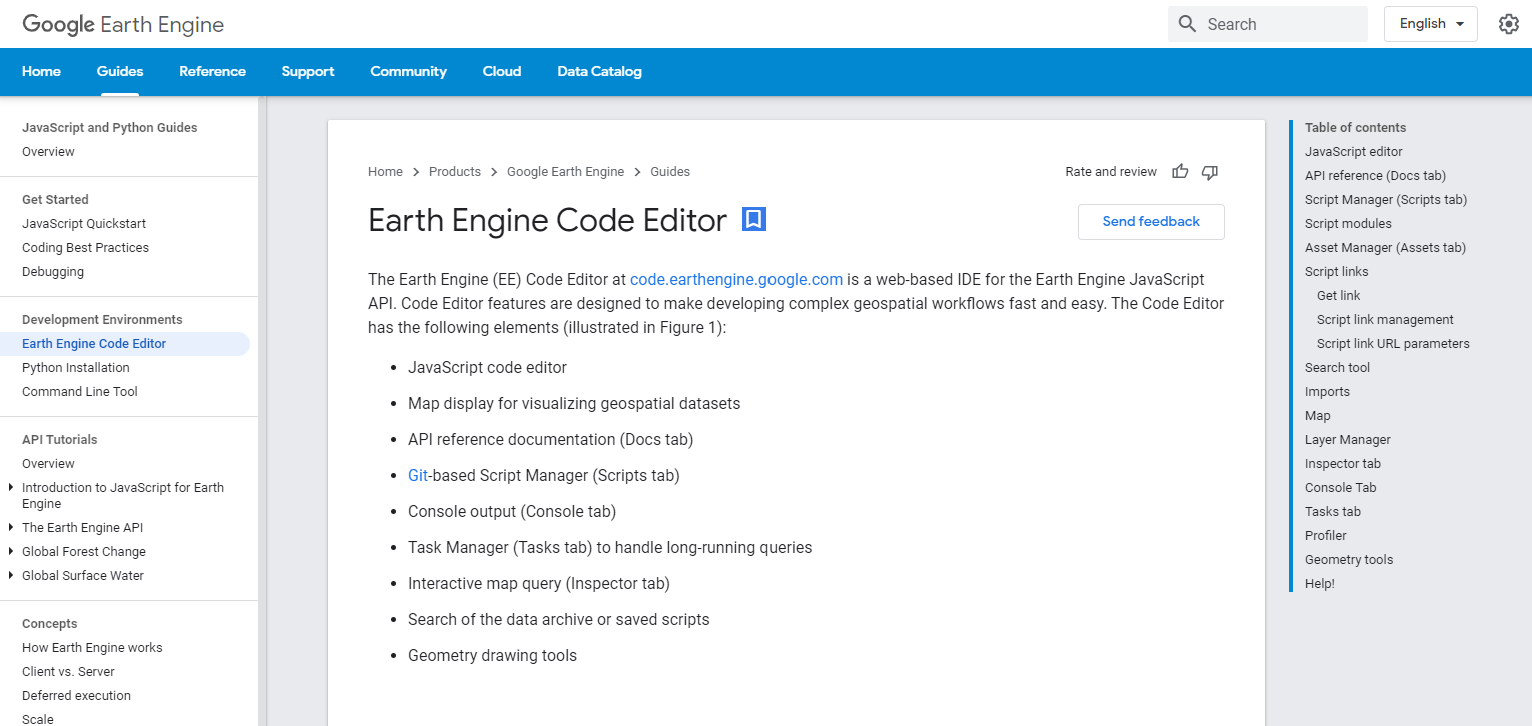
\includegraphics[width=0.8\linewidth]{clip_image001} \caption{A view of the google earth engine code editor}\label{fig:code-editor}
\end{figure}

\hypertarget{features-and-feature-collections}{%
\subsection{Features and Feature Collections}\label{features-and-feature-collections}}

\hypertarget{features}{%
\subsubsection{Features}\label{features}}

At the most basic definition, a Feature in GEE is an object which stores a \texttt{geometry} property (\texttt{Point}, \texttt{Line}, \texttt{Polygon}) along with it's associated properties. GEE uses the GeoJSON format to store and transmit these features. In the previous video, we saw how to build geometries within Google Earth Engine, a feature adds meaningful information to it. This would be a good section to review working with dictionaries with JavaScript.

Let's say we created an individual point, which we want to associate with data that we collected. The first line establishes the variable \texttt{point}, which is then used as the \texttt{geometry} to create a \texttt{feature}. The curly braces represent a JavaScript dictionary, which creates Key:Value pairs, which in our case is the type of tree and a measurement of the size. this new variable, \texttt{treeFeature}, now contains geographic information along with attribute data about that point.

\begin{Shaded}
\begin{Highlighting}[]
\CommentTok{// geometry created from within GEE}
\KeywordTok{var}\NormalTok{ point }\OperatorTok{=} \VariableTok{ee}\NormalTok{.}\VariableTok{Geometry}\NormalTok{.}\AttributeTok{Point}\NormalTok{([}\OperatorTok{-}\FloatTok{79.68}\OperatorTok{,} \FloatTok{42.06}\NormalTok{])}\OperatorTok{;}
\CommentTok{// Create a Feature from the geometry}
\KeywordTok{var}\NormalTok{ treeFeature }\OperatorTok{=} \VariableTok{ee}\NormalTok{.}\AttributeTok{Feature}\NormalTok{(point}\OperatorTok{,} \OperatorTok{\{}\DataTypeTok{type}\OperatorTok{:} \StringTok{'Pine'}\OperatorTok{,} \DataTypeTok{size}\OperatorTok{:} \DecValTok{15}\OperatorTok{\}}\NormalTok{)}\OperatorTok{;}
\end{Highlighting}
\end{Shaded}

Obviously this is just one point, but JavaScript and GEE engine provide functionality for bringing different data sources together and automatically associating geometries with attribute data. This can be done within GEE or outside, depending on your preferences.

\hypertarget{feature-collections}{%
\subsubsection{Feature Collections}\label{feature-collections}}

Just like the relationship between images and image collections, Feature Collections are Features that can be grouped together for ease of use and analysis. They can be different types and combinations of geometry, as well as associated tabular data. The code segment from the documentation consolidates the operations discussed earlier. Each line has an interior layer which creates the geometry (\texttt{ee.Geometry.-\/-\/-()} ), which is then associated with attribute data (information within the \{\} ) and then converted to a Feature. This variable is a JavaScript\texttt{list}, which contains three separate features. This is then converted to a Feature Collection with the command \texttt{ee.FeatureCollection(features)}

\begin{Shaded}
\begin{Highlighting}[]
\CommentTok{// Make a list of Features.}
\KeywordTok{var}\NormalTok{ features }\OperatorTok{=}\NormalTok{ [}
  \VariableTok{ee}\NormalTok{.}\AttributeTok{Feature}\NormalTok{(}\VariableTok{ee}\NormalTok{.}\VariableTok{Geometry}\NormalTok{.}\AttributeTok{Rectangle}\NormalTok{(}\FloatTok{30.01}\OperatorTok{,} \FloatTok{59.80}\OperatorTok{,} \FloatTok{30.59}\OperatorTok{,} \FloatTok{60.15}\NormalTok{)}\OperatorTok{,} \OperatorTok{\{}\DataTypeTok{name}\OperatorTok{:} \StringTok{'Voronoi'}\OperatorTok{\}}\NormalTok{)}\OperatorTok{,}
  \VariableTok{ee}\NormalTok{.}\AttributeTok{Feature}\NormalTok{(}\VariableTok{ee}\NormalTok{.}\VariableTok{Geometry}\NormalTok{.}\AttributeTok{Point}\NormalTok{(}\OperatorTok{-}\FloatTok{73.96}\OperatorTok{,} \FloatTok{40.781}\NormalTok{)}\OperatorTok{,} \OperatorTok{\{}\DataTypeTok{name}\OperatorTok{:} \StringTok{'Thiessen'}\OperatorTok{\}}\NormalTok{)}\OperatorTok{,}
  \VariableTok{ee}\NormalTok{.}\AttributeTok{Feature}\NormalTok{(}\VariableTok{ee}\NormalTok{.}\VariableTok{Geometry}\NormalTok{.}\AttributeTok{Point}\NormalTok{(}\FloatTok{6.4806}\OperatorTok{,} \FloatTok{50.8012}\NormalTok{)}\OperatorTok{,} \OperatorTok{\{}\DataTypeTok{name}\OperatorTok{:} \StringTok{'Dirichlet'}\OperatorTok{\}}\NormalTok{)}
\NormalTok{]}\OperatorTok{;}

\CommentTok{// Create a FeatureCollection from the list and print it.}
\KeywordTok{var}\NormalTok{ fromList }\OperatorTok{=} \VariableTok{ee}\NormalTok{.}\AttributeTok{FeatureCollection}\NormalTok{(features)}\OperatorTok{;}
\AttributeTok{print}\NormalTok{(fromList)}\OperatorTok{;}
\end{Highlighting}
\end{Shaded}

If you take this code block and run it in Google Earth Engine, you can see the information that is contained within the FeatureCollection, which has three elements (Features) and two columns (the \texttt{index} and the \texttt{properties}). By clicking on the dropdown next to each one, you can see that the first feature is a Polygon that has the name of `Voronoi'.

\begin{center}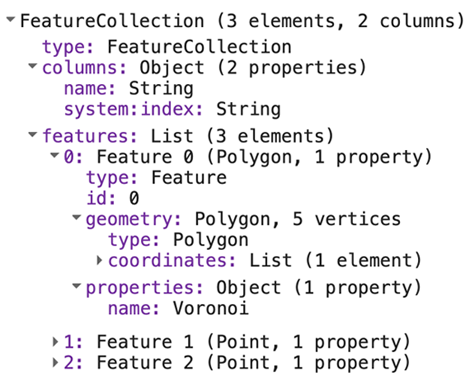
\includegraphics[width=0.5\linewidth]{im2} \end{center}

Once you have information in a Feature Collection, you can filter it to find specific information, such as the name of an object or based on the size of a polygon, or provide aggregated analysis. The \href{https://developers.google.com/earth-engine/guides/features}{documentation} on working with Feature Collections is comprehensive, and provides many ideas on how to use them efficiently in in your analysis.

\hypertarget{methods-reducers}{%
\subsection{Methods: Reducers}\label{methods-reducers}}

Up until now, we have focused on objects: Images, Features, and Geometries. Reducers are a method of aggregating data for analysis. For instance, we could take an Image Collection and use \texttt{reducer} to find the average value at each pixel, resulting in a single layer. Or we could reduce an image to a set of regions, grouping similar data together to create a simplifed map. The applications of Reducer are endless, and can be applied to both Images and Features. There are different functions for different object types, and Reducer can be both combined and sequenced to create a chain of analysis. From the documentation, the code chunk below creates the variable \texttt{collection} which is a collection that is filtered to the year 2016 and defined to a specific point. The variable \texttt{extrema} then reduces the dataset to identify the minimum and maximum value at that specific point for every band.

\begin{Shaded}
\begin{Highlighting}[]
\CommentTok{// Load and filter the Sentinel-2 image collection.}
\KeywordTok{var}\NormalTok{ collection }\OperatorTok{=} \VariableTok{ee}\NormalTok{.}\AttributeTok{ImageCollection}\NormalTok{(}\StringTok{'COPERNICUS/S2'}\NormalTok{)}
\NormalTok{    .}\AttributeTok{filterDate}\NormalTok{(}\StringTok{'2016-01-01'}\OperatorTok{,} \StringTok{'2016-12-31'}\NormalTok{)}
\NormalTok{    .}\AttributeTok{filterBounds}\NormalTok{(}\VariableTok{ee}\NormalTok{.}\VariableTok{Geometry}\NormalTok{.}\AttributeTok{Point}\NormalTok{([}\OperatorTok{-}\FloatTok{81.31}\OperatorTok{,} \FloatTok{29.90}\NormalTok{]))}\OperatorTok{;}
\CommentTok{// Reduce the collection.}
\KeywordTok{var}\NormalTok{ extrema }\OperatorTok{=} \VariableTok{collection}\NormalTok{.}\AttributeTok{reduce}\NormalTok{(}\VariableTok{ee}\NormalTok{.}\VariableTok{Reducer}\NormalTok{.}\AttributeTok{minMax}\NormalTok{())}\OperatorTok{;}
\end{Highlighting}
\end{Shaded}

If you print \texttt{extrema} in the console, you can see that the result is 32 separate `bands', which represents the minimum and maximum value for all 16 bands in the Sentinel data. In the screenshot below, you can expand the first `band', which identifies the attributes of the minimum value of Band 1.

\begin{center}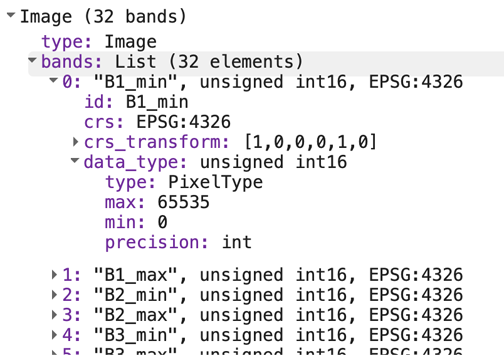
\includegraphics[width=0.5\linewidth]{im3} \end{center}

There are hundreds of different operations for using \texttt{Reducer}, with the functions listed on the left hand table under `Docs'. Certain functions will only work with specific object types, but follow along with the Reducer \href{https://developers.google.com/earth-engine/guides/reducers_intro}{documentation} to get a better understanding of how to aggregate data and extract meaningful results. Getting familiar with Reducer is an essential component to working with Google Earth Engine.

\begin{center}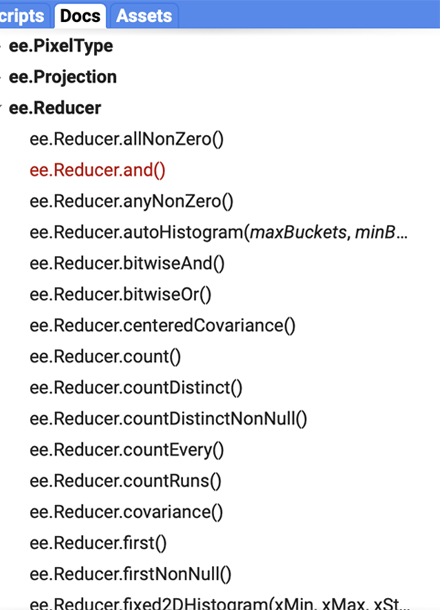
\includegraphics[width=0.5\linewidth]{im4} \end{center}

\hypertarget{joins-and-arrays}{%
\subsection{Joins and Arrays}\label{joins-and-arrays}}

\hypertarget{join}{%
\subsubsection{Join}\label{join}}

If you have programmed in the past, joining data togetgher is likely a familiar concept. This process assicates information from one set of data with relevant data from another set on a specific attribute. Let's say you have an Image Collection of Landsat data that is filtered to the first six months of the year 2016 and a bounding box of your area of study. You also have a table of Redwood tree locations that is filtered to the same area of study, although it contains information over the past decade. You can use a Join to associate information about the trees from the Feature Collection and include it in the Image Collection, keeping only the relevant data. You now have a dataset with useful information from both the Image Collection and Feature Collection in one location. Although there are different types of joins, the process brings information together, keeping only relevant information. The \href{https://developers.google.com/earth-engine/guides/joins_save_all}{documentation} on Joins goes over specific examples and concepts, but a crucial component is understanding the type of join you need the three most prominent within GEE are:

\begin{itemize}
\tightlist
\item
  Left Join

  \begin{itemize}
  \tightlist
  \item
    Keeps all the information from the primary dataset, and only information that joins from the secondary datset
  \end{itemize}
\item
  Inner Join

  \begin{itemize}
  \tightlist
  \item
    Keeps only the information where the primary and secondary data match
  \end{itemize}
\item
  Spatial Join

  \begin{itemize}
  \tightlist
  \item
    A join based on spatial location (ie, keep only the geometry points that fall within a specified buffer)
  \end{itemize}
\end{itemize}

GEE provides some unique types of joins, including `Save-All', `Save-Best' and `Save-First', which are useful if you want to look at a specific area.

\hypertarget{arrays}{%
\subsubsection{Arrays}\label{arrays}}

Arrays are a collection of data where information is stored contiguously - matrices are a multi-dimensional array. For instance, an image might have 1024 rows and 1024 columns. Each row is an array, each column is an array, and taken together, you have a 2-dimensional array, also known as a matrix. If the image has three separate color channels, then that is a 3-dimensional array. Some of the terminology changes depending on discipline (ie, physics vs.~computer science), but if you are familiar with working with matrices and arrays in programming languages such as Matlab or OpenCV, it is important to understand the role of arrays within GEE.

In fact, Google Earth Engine states that working with arrays outside of the established functions that they have built is not recommended, as GEE is not specifically designed for array-based math, and will lead to unoptimized performance.

There is a very informative \href{https://developers.google.com/earth-engine/guides/arrays_intro}{video} that delves into the engineering behind Google Earth Engine, but in this course we will only be doing a limited amount with array transformations and Eigen Analysis. In many cases, you will probably be better off aggregating the specific data and then conducting array mathematics with programming frameworks geared to that context.

\hypertarget{additional-resources}{%
\subsection{Additional Resources}\label{additional-resources}}

\begin{itemize}
\tightlist
\item
  Google Earth Engine \href{https://earthengine.google.com}{link}
\item
  Code Editor \href{https://developers.google.com/earth-engine/guides/playground?hl=en}{Map} -- what all the features on the code editor mean
\item
  \href{https://developers.google.com/earth-engine/datasets/}{Datasets}
\item
  \href{https://earthengine.google.com/case_studies/}{Case Studies}
\item
  Google Earth Engine \href{https://medium.com/google-earth}{Blog}
\item
  \href{https://developers.google.com/earth-engine/tutorials/tutorials}{Video} tutorials on using GEE (from the Earth Engine Users' Summit)
\end{itemize}

\hypertarget{lab1}{%
\section{Remote Sensing Background}\label{lab1}}

\hypertarget{overview-1}{%
\subsection*{Overview}\label{overview-1}}
\addcontentsline{toc}{subsection}{Overview}

The purpose of this lab is to introduce digital images, datum, and projections, as well as demonstrate concepts of spatial, spectral, temporal and radiometric resolution. You will be introduced to image data from several sensors aboard various platforms. At the completion of the lab, you will be able to understand the difference between remotely sensed datasets based on sensor characteristics and how to choose an appropriate dataset based on these concepts.

\hypertarget{learning-outcomes-1}{%
\paragraph{Learning Outcomes}\label{learning-outcomes-1}}
\addcontentsline{toc}{paragraph}{Learning Outcomes}

\begin{enumerate}
\def\labelenumi{\arabic{enumi}.}
\tightlist
\item
  Describe the following terms:

  \begin{itemize}
  \tightlist
  \item
    Digital image
  \item
    Datum
  \item
    Projection
  \item
    Resolution (spatial, spectral, temporal, radiometric)
  \end{itemize}
\item
  Navigate the Google Earth Engine console to gather information about a digital image
\item
  Evaluate the projection and attributes of a digital image
\item
  Apply image visualization code in GEE to visualize a digital image
\end{enumerate}

\hypertarget{what-is-a-digital-image}{%
\subsection{What is a digital image?}\label{what-is-a-digital-image}}

A digital image is a matrix of same-sized pixels that are each defined by two main attributes: (1) the position, as defined by rows and columns and (2) the a value associated with that position.

A digital image 8 pixels wide by 8 pixels tall could thus look like the image below. Note though you can reference the position from a given axis, typically, image processing uses the top-left of an image as the reference point, as in the below image.

\begin{figure}

{\centering 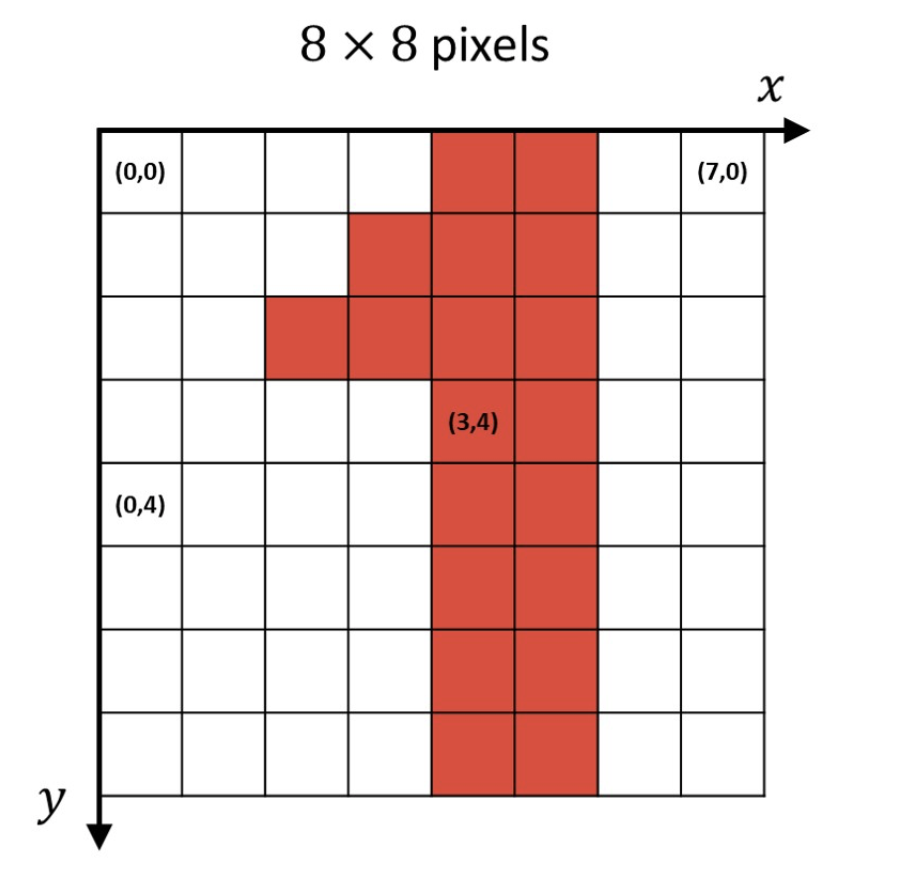
\includegraphics[width=0.5\linewidth]{clip_image003} 

}

\caption{Digital Image Example}\label{fig:digimage}
\end{figure}

A ``traditional'' optical photograph typically represents three layers (often the brightness values represented in the Red, Blue, and Green portions of the electromagnetic spectrum). Together, these three layers create a full-color photograph that is represented by a three dimensional matrix where pixel position is characterized by the (1) row (2) column (3) \emph{and} layer.

Digital images are also often called \href{https://en.wikipedia.org/wiki/Raster_graphics}{rasters}, and ESRI has a great overview of rasters used in geospatial analysis featured \href{https://desktop.arcgis.com/en/arcmap/10.3/manage-data/raster-and-images/what-is-raster-data.htm}{here}.

\hypertarget{from-digital-image-to-geospatial-image}{%
\subsubsection{From digital image to geospatial image}\label{from-digital-image-to-geospatial-image}}

A digital image is a flat, square surface. However, the earth is round (spherical).

Thus to make use of the synoptic properties of remote sensing data, we need to align the pixels in our image to a real-world location. There's quite a bit of mathematics involved in this process, but we will focus on two main components - establishing a Geographic Coordinate System (GCS) and a Projected Coordinate System (PCS).

The GCS defines the spherical location of the image whereas the PCS defines how the grid around that location is constructed. Because the earth is not a perfect sphere, there are different GCS for different regions, such as `North American Datum: 83' which is used to accurately define North America, and `World Geodetic System of 1984', which is used globally.

The PCS then constructs a flat grid around the GCS in which you can create a relationship between each pixel of a 2-dimensional image to the corresponding area on the world. Some of the common PCS formats include EPSG, Albers Conic, Lambert, Eckert, Equidistant, etc. Different types of PCS's are designed for different formats, as the needs of a petroleum engineer working over a few square miles will differ from than a climate change researcher at the scope of the planet, for example.

ESRI (the makers of ArcGIS) has an \href{https://www.esri.com/arcgis-blog/products/arcgis-pro/mapping/gcs_vs_pcs/}{article} discussing the difference between GCS and PCS that provides further context. While you should be aware of the differences between GCS and PCS's -- especially when you intend to run analyses on the data you download from GEE in another system such as R, Python, or Arc -- GEE takes care of much of the complexity of these differences behind the scenes. Further documentation on the GEE methodology can be found \href{https://developers.google.com/earth-engine/guides/projections}{here}. In our first exercise, we will show you how to identify the PCS so you can understand the underlying structure.

Furthermore, remote sensing data often consists of more than the three Red-Green-Bluye layers we're used to seeing visualized in traditional photography. For instance, the Landsat 8 sensor has eleven bands capturing information from eleven different portions of the electromagentic spectrum, including near infrared (NIR) and thermal bands that are invisible to the human eye. Many Machine Learning projects also involve normalizing or transforming the information contained within each of these layers, which we will return to in subsequent labs.

In sum, understanding the bands available in your datasets, identifying which bands are necessary (and appropriate) for your analysis, and ensuring that these data represent consistent spatial locations is essential. While GEE simplifies many complex calculations behind the scenes, this lab will help us unpack the products available to us and their essential characteristics.

\hypertarget{summary}{%
\paragraph{Summary}\label{summary}}
\addcontentsline{toc}{paragraph}{Summary}

Each pixel has a position, measured with respect to the axes of some coordinate reference system (CRS), such as a \href{https://en.wikipedia.org/wiki/Geographic_coordinate_system}{geographic coordinate system}. A CRS in Earth Engine is often referred to as a projection, since it combines a shape of the Earth with a \href{https://en.wikipedia.org/wiki/Geodetic_datum}{datum} and a transformation from that spherical shape to a flat map, called a \href{https://en.wikipedia.org/wiki/Map_projection}{projection}.

\begin{figure}

{\centering 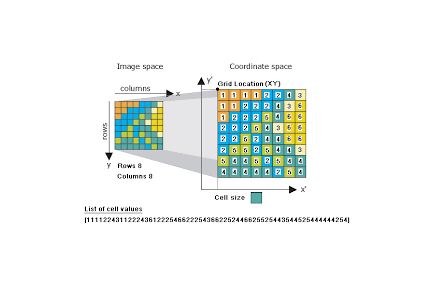
\includegraphics[width=0.8\linewidth]{clip_image002} 

}

\caption{A pixel, raster, and a CRS}\label{fig:pixel}
\end{figure}

\hypertarget{visualize-a-digital-image}{%
\subsubsection{Visualize a Digital Image}\label{visualize-a-digital-image}}

Let's view a digital image in GEE to better understand this concept:

\begin{enumerate}
\def\labelenumi{\arabic{enumi}.}
\item
  In the map window of GEE, click on the Point geometry tool using the \href{https://developers.google.com/earth-engine/playground\#geometry-tools}{geometry drawing tools} to define your area of interest (for the purposes of consistency in this exercise, place a point on the Virginia Tech Drillfield, which will bring you roughly to
  \texttt{{[}-80.42,37.23{]}}). As a reminder, you can find more information on geometry drawing tools in GEE's Guides. Name the import \texttt{point}.
\item
  Import NAIP imagery by searching for `naip' and choosing the \emph{`NAIP: National Agriculture Imagery Program'} raster dataset. Name the import \texttt{naip}.
\item
  Get a single, recent NAIP image over your study area and inspect it:

\begin{Shaded}
\begin{Highlighting}[]
\CommentTok{//  Get a single NAIP image over the area of interest.  }
\KeywordTok{var}\NormalTok{  image }\OperatorTok{=} \VariableTok{ee}\NormalTok{.}\AttributeTok{Image}\NormalTok{(naip  }
\NormalTok{                      .}\AttributeTok{filterBounds}\NormalTok{(point)}
\NormalTok{                      .}\AttributeTok{sort}\NormalTok{(}\StringTok{'system:time_start'}\OperatorTok{,} \KeywordTok{false}\NormalTok{)}
\NormalTok{                      .}\AttributeTok{first}\NormalTok{())}\OperatorTok{;}      
\CommentTok{//  Print the image to the console.  }
\AttributeTok{print}\NormalTok{(}\StringTok{'Inspect the image object:'}\OperatorTok{,}\NormalTok{ image)}\OperatorTok{;}     
\CommentTok{//  Display the image with the default visualization.  }
\VariableTok{Map}\NormalTok{.}\AttributeTok{centerObject}\NormalTok{(point}\OperatorTok{,} \DecValTok{18}\NormalTok{)}\OperatorTok{;}  
\VariableTok{Map}\NormalTok{.}\AttributeTok{addLayer}\NormalTok{(image}\OperatorTok{,} \OperatorTok{\{\},} \StringTok{'Original image'}\NormalTok{)}\OperatorTok{;}
\end{Highlighting}
\end{Shaded}
\item
  Expand the image object that is printed to the console by clicking on the dropdown triangles. Expand the property called \texttt{bands} and expand one of the bands (0, for example). Note that the CRS transform is stored in the \texttt{crs\_transform} property underneath the band dropdown and the CRS is stored in the \texttt{crs} property, which references an EPSG code.

  \begin{quote}
  \textbf{EPSG Codes} are 4-5 digit numbers that represent CRS definitions. The acronym EPGS, comes from the (now defunct) European Petroleum Survey Group. The CRS of this image is \href{https://spatialreference.org/ref/epsg/nad83-utm-zone-17n/}{EPSG:26917}. You can often learn more about those \href{http://www.epsg-registry.org/}{EPSG codes} from \href{http://spatialreference.org/}{thespatialreference.org} or from the \href{https://epsg.org/home.html}{ESPG homepage}.
  \end{quote}

  \begin{quote}
  The CRS transform is a list \texttt{{[}m00,\ m01,\ m02,\ m10,\ m11,\ m12{]}} in the notation of \href{http://docs.oracle.com/javase/7/docs/api/java/awt/geom/AffineTransform.html}{this reference}. The CRS transform defines how to map pixel coordinates to their associated spherical coordinate through an affine transformation. While affine transformations are beyond the scope of this class, more information can be found at \href{https://rasterio.readthedocs.io/en/latest/topics/georeferencing.html}{Rasterio}, which provides detailed documentation for the popular Python library designed for working with geospatial data.
  \end{quote}
\item
  In addition to using the dropdowns, you can also access these data programmatically with the \texttt{.projection()} method:

\begin{Shaded}
\begin{Highlighting}[]
\CommentTok{// Display the projection of band 0}
\AttributeTok{print}\NormalTok{(}\StringTok{'Inspect the projection of band 0:'}\OperatorTok{,} \VariableTok{image}\NormalTok{.}\AttributeTok{select}\NormalTok{(}\DecValTok{0}\NormalTok{).}\AttributeTok{projection}\NormalTok{())}\OperatorTok{;}
\end{Highlighting}
\end{Shaded}
\item
  Note that the projection can differ by band, which is why it's good practice to inspect the projection of individual image bands.
\item
  (If you call \texttt{.projection()} on an image for which the projection differs by band, you'll get an error.) Exchange the NAIP imagery with the Planet SkySat MultiSpectral image collection, and note that the error occurs because the `P' band has a different pixel size than the others.
\item
  Explore the \texttt{ee.Projection} docs to learn about useful methods offered by the \texttt{Projection} object. To play with projections offline, try \href{http://www.giss.nasa.gov/tools/gprojector/}{this tool}.
\end{enumerate}

\hypertarget{digital-image-visualization-and-stretching}{%
\subsubsection{Digital Image Visualization and Stretching}\label{digital-image-visualization-and-stretching}}

You've learned about how an image stores pixel data in each band as digital numbers (DNs) and how the pixels are organized spatially. When you add an image to the map, Earth Engine handles the spatial display for you by recognizing the projection and putting all the pixels in the right place. However, you must specify how to stretch the DNs to make an 8-bit display image (e.g., the \texttt{min} and \texttt{max} visualization parameters). Specifying \texttt{min} and \texttt{max} applies (where DN' is the displayed value):

\[ DN' =   \frac{ 255 (DN - min)}{(max - min)} \]

\begin{enumerate}
\def\labelenumi{\arabic{enumi}.}
\item
  To apply a \href{https://en.wikipedia.org/wiki/Gamma_correction}{gamma correction} (DN' = DN\(_\gamma\)), use:

\begin{Shaded}
\begin{Highlighting}[]
\CommentTok{// Display gamma stretches of the input image.}
\VariableTok{Map}\NormalTok{.}\AttributeTok{addLayer}\NormalTok{(}\VariableTok{image}\NormalTok{.}\AttributeTok{visualize}\NormalTok{(}\OperatorTok{\{}\DataTypeTok{gamma}\OperatorTok{:} \FloatTok{0.5}\OperatorTok{\}}\NormalTok{)}\OperatorTok{,} \OperatorTok{\{\},} \StringTok{'gamma = 0.5'}\NormalTok{)}\OperatorTok{;}
\VariableTok{Map}\NormalTok{.}\AttributeTok{addLayer}\NormalTok{(}\VariableTok{image}\NormalTok{.}\AttributeTok{visualize}\NormalTok{(}\OperatorTok{\{}\DataTypeTok{gamma}\OperatorTok{:} \FloatTok{1.5}\OperatorTok{\}}\NormalTok{)}\OperatorTok{,} \OperatorTok{\{\},} \StringTok{'gamma = 1.5'}\NormalTok{)}\OperatorTok{;}
\end{Highlighting}
\end{Shaded}

  Note that gamma is supplied as an argument to \href{https://developers.google.com/earth-engine/apidocs/ee-image-visualize}{image.visualize()} so that you can click on the map to see the difference in pixel values (try it!). It's possible to specify \texttt{gamma}, \texttt{min}, and \texttt{max} to achieve other unique visualizations.
\item
  To apply a \href{https://en.wikipedia.org/wiki/Histogram_equalization}{histogram equalization} stretch, use the \href{https://devsite.googleplex.com/earth-engine/image_visualization\#styled-layer-descriptors}{\texttt{sldStyle()}} method

\begin{Shaded}
\begin{Highlighting}[]
\CommentTok{// Define a RasterSymbolizer element with '_enhance_' for a placeholder.}
  \KeywordTok{var}\NormalTok{ histogram_sld }\OperatorTok{=}
    \StringTok{'<RasterSymbolizer>'} \OperatorTok{+}
      \StringTok{'<ContrastEnhancement><Histogram/></ContrastEnhancement>'} \OperatorTok{+}
      \StringTok{'<ChannelSelection>'} \OperatorTok{+}
        \StringTok{'<RedChannel>'} \OperatorTok{+}
          \StringTok{'<SourceChannelName>R</SourceChannelName>'} \OperatorTok{+}
        \StringTok{'</RedChannel>'} \OperatorTok{+}
        \StringTok{'<GreenChannel>'} \OperatorTok{+}
          \StringTok{'<SourceChannelName>G</SourceChannelName>'} \OperatorTok{+}
        \StringTok{'</GreenChannel>'} \OperatorTok{+}
        \StringTok{'<BlueChannel>'} \OperatorTok{+}
          \StringTok{'<SourceChannelName>B</SourceChannelName>'} \OperatorTok{+}
        \StringTok{'</BlueChannel>'} \OperatorTok{+}
      \StringTok{'</ChannelSelection>'} \OperatorTok{+}
    \StringTok{'</RasterSymbolizer>'}\OperatorTok{;}

  \CommentTok{// Display the image with a histogram equalization stretch.}
  \VariableTok{Map}\NormalTok{.}\AttributeTok{addLayer}\NormalTok{(}\VariableTok{image}\NormalTok{.}\AttributeTok{sldStyle}\NormalTok{(histogram_sld)}\OperatorTok{,} \OperatorTok{\{\},} \StringTok{'Equalized'}\NormalTok{)}\OperatorTok{;}
\end{Highlighting}
\end{Shaded}

  The \href{https://devsite.googleplex.com/earth-engine/image_visualization\#styled-layer-descriptors}{\texttt{sldStyle()}} method requires image statistics to be computed in a region (to determine the histogram).
\end{enumerate}

\hypertarget{spatial-resolution}{%
\subsection{Spatial Resolution}\label{spatial-resolution}}

In the present context, spatial resolution often means pixel size. In practice, spatial resolution depends on the projection of the sensor's instantaneous field of view (IFOV) on the ground and how a set of radiometric measurements are resampled into a regular grid. To see the difference in spatial resolution resulting from different sensors, let's visualize data at different scales from different sensors.

\hypertarget{modis}{%
\subsubsection{MODIS}\label{modis}}

There are two Moderate Resolution Imaging Spectro-Radiometers (\href{http://modis.gsfc.nasa.gov/}{MODIS}) aboard the \href{http://terra.nasa.gov/}{Terra} and \href{http://aqua.nasa.gov/}{Aqua} satellites. Different MODIS \href{http://modis.gsfc.nasa.gov/about/specifications.php}{bands} produce data at different spatial resolutions. For the visible bands, the lowest common resolution is 500 meters (red and NIR are 250 meters). Data from the MODIS platforms are used to produce a large number of data sets having daily, weekly, 16-day, monthly, and annual data sets. Outside this lab, you can find a list of MODIS land products \href{https://lpdaac.usgs.gov/dataset_discovery/modis/modis_products_table}{here}.

\begin{enumerate}
\def\labelenumi{\arabic{enumi}.}
\item
  Search for `\href{https://lpdaac.usgs.gov/dataset_discovery/modis/modis_products_table/myd09ga_v006}{MYD09GA}' and import `\emph{MYD09GA.006 Aqua Surface Reflectance Daily Global 1km and 500m}'. Name the import \texttt{myd09}.
\item
  Zoom the map to San Francisco (SFO) airport:

\begin{Shaded}
\begin{Highlighting}[]
\CommentTok{// Define a region of interest as a point at SFO airport.}
\KeywordTok{var}\NormalTok{ sfoPoint }\OperatorTok{=} \VariableTok{ee}\NormalTok{.}\VariableTok{Geometry}\NormalTok{.}\AttributeTok{Point}\NormalTok{(}\OperatorTok{-}\FloatTok{122.3774}\OperatorTok{,} \FloatTok{37.6194}\NormalTok{)}\OperatorTok{;}

\CommentTok{// Center the map at that point.}
\VariableTok{Map}\NormalTok{.}\AttributeTok{centerObject}\NormalTok{(sfoPoint}\OperatorTok{,} \DecValTok{16}\NormalTok{)}\OperatorTok{;}
\end{Highlighting}
\end{Shaded}
\item
  To display a false-color MODIS image, select an image acquired by the Aqua MODIS sensor and display it for SFO:

\begin{Shaded}
\begin{Highlighting}[]
\CommentTok{// Get a surface reflectance image from the MODIS MYD09GA collection.}
\KeywordTok{var}\NormalTok{ modisImage }\OperatorTok{=} \VariableTok{ee}\NormalTok{.}\AttributeTok{Image}\NormalTok{(}\VariableTok{myd09}\NormalTok{.}\AttributeTok{filterDate}\NormalTok{(}\StringTok{'2017-07-01'}\NormalTok{).}\AttributeTok{first}\NormalTok{())}\OperatorTok{;}

\CommentTok{// Use these MODIS bands for red, green, blue, respectively.}
\KeywordTok{var}\NormalTok{ modisBands }\OperatorTok{=}\NormalTok{ [}\StringTok{'sur_refl_b01'}\OperatorTok{,} \StringTok{'sur_refl_b04'}\OperatorTok{,} \StringTok{'sur_refl_b03'}\NormalTok{]}\OperatorTok{;}

\CommentTok{// Define visualization parameters for MODIS.}
\KeywordTok{var}\NormalTok{ modisVis }\OperatorTok{=} \OperatorTok{\{}\DataTypeTok{bands}\OperatorTok{:}\NormalTok{ modisBands}\OperatorTok{,} \DataTypeTok{min}\OperatorTok{:} \DecValTok{0}\OperatorTok{,} \DataTypeTok{max}\OperatorTok{:} \DecValTok{3000}\OperatorTok{\};}

\CommentTok{// Add the MODIS image to the map}
\VariableTok{Map}\NormalTok{.}\AttributeTok{addLayer}\NormalTok{(modisImage}\OperatorTok{,}\NormalTok{ modisVis}\OperatorTok{,} \StringTok{'MODIS'}\NormalTok{)}\OperatorTok{;}
\end{Highlighting}
\end{Shaded}
\item
  Note the size of pixels with respect to objects on the ground. (It may help to turn on the satellite basemap to see high-resolution data for comparison.) Print the size of the pixels (in meters) with:

\begin{Shaded}
\begin{Highlighting}[]
\CommentTok{// Get the scale of the data from the first band's projection:}
\KeywordTok{var}\NormalTok{ modisScale }\OperatorTok{=} \VariableTok{modisImage}\NormalTok{.}\AttributeTok{select}\NormalTok{(}\StringTok{'sur_refl_b01'}\NormalTok{)}
\NormalTok{.}\AttributeTok{projection}\NormalTok{().}\AttributeTok{nominalScale}\NormalTok{()}\OperatorTok{;}

\AttributeTok{print}\NormalTok{(}\StringTok{'MODIS scale:'}\OperatorTok{,}\NormalTok{ modisScale)}\OperatorTok{;}
\end{Highlighting}
\end{Shaded}
\item
  Note these \texttt{MYD09} data are surface reflectance scaled by 10000 (not TOA reflectance), meaning that clever NASA scientists have done a fancy atmospheric correction for you!
\end{enumerate}

\hypertarget{multispectral-scanners}{%
\subsubsection{Multispectral Scanners}\label{multispectral-scanners}}

Multi-spectral scanners were flown aboard Landsats 1-5. (\href{https://landsat.gsfc.nasa.gov/multispectral-scanner-system}{MSS}) data have a spatial resolution of 60 meters.

\begin{enumerate}
\def\labelenumi{\arabic{enumi}.}
\item
  Search for `landsat 5 mss' and import the result called \emph{`USGS Landsat 5 MSS Collection 1 Tier 2 Raw Scenes'}. Name the import \texttt{mss}.
\item
  To visualize MSS data over SFO (for a relatively cloud-free) image, use:

\begin{Shaded}
\begin{Highlighting}[]
\CommentTok{// Filter MSS imagery by location, date and cloudiness.   }
\KeywordTok{var}\NormalTok{ mssImage }\OperatorTok{=} \VariableTok{ee}\NormalTok{.}\AttributeTok{Image}\NormalTok{(mss     }
\NormalTok{                        .}\AttributeTok{filterBounds}\NormalTok{(}\VariableTok{Map}\NormalTok{.}\AttributeTok{getCenter}\NormalTok{())     }
\NormalTok{                        .}\AttributeTok{filterDate}\NormalTok{(}\StringTok{'2011-05-01'}\OperatorTok{,}  \StringTok{'2011-10-01'}\NormalTok{)     }
\NormalTok{                        .}\AttributeTok{sort}\NormalTok{(}\StringTok{'CLOUD_COVER'}\NormalTok{)     }
                        \CommentTok{//  Get the least cloudy image.     }
\NormalTok{                        .}\AttributeTok{first}\NormalTok{())}\OperatorTok{;}  

\CommentTok{// Display the MSS image as a color-IR composite.}
\VariableTok{Map}\NormalTok{.}\AttributeTok{addLayer}\NormalTok{(mssImage}\OperatorTok{,} \OperatorTok{\{}\DataTypeTok{bands}\OperatorTok{:}\NormalTok{ [}\StringTok{'B3'}\OperatorTok{,} \StringTok{'B2'}\OperatorTok{,} \StringTok{'B1'}\NormalTok{]}\OperatorTok{,} \DataTypeTok{min}\OperatorTok{:} \DecValTok{0}\OperatorTok{,} \DataTypeTok{max}\OperatorTok{:} \DecValTok{200}\OperatorTok{\},} \StringTok{'MSS'}\NormalTok{)}\OperatorTok{;}
\end{Highlighting}
\end{Shaded}
\item
  Check the scale (in meters) as before:

\begin{Shaded}
\begin{Highlighting}[]
\CommentTok{// Get the scale of the MSS data from its projection:}
\KeywordTok{var}\NormalTok{ mssScale }\OperatorTok{=} \VariableTok{mssImage}\NormalTok{.}\AttributeTok{select}\NormalTok{(}\StringTok{'B1'}\NormalTok{).}\AttributeTok{projection}\NormalTok{().}\AttributeTok{nominalScale}\NormalTok{()}\OperatorTok{;}
\AttributeTok{print}\NormalTok{(}\StringTok{'MSS scale:'}\OperatorTok{,}\NormalTok{ mssScale)}\OperatorTok{;}
\end{Highlighting}
\end{Shaded}
\end{enumerate}

\hypertarget{thematic-mapper-tm}{%
\subsubsection{Thematic Mapper (TM)}\label{thematic-mapper-tm}}

The Thematic Mapper (\href{https://landsat.gsfc.nasa.gov/landsat-4-5/tm}{TM}) was flown aboard Landsats 4-5. (It was succeeded by the Enhanced Thematic Mapper (\href{https://landsat.gsfc.nasa.gov/about/enhanced-thematic-mapper}{ETM+}) aboard Landsat 7 and the Operational Land Imager (\href{https://landsat.gsfc.nasa.gov/landsat-8/operational-land-imager}{OLI}) / Thermal Infrared Sensor (\href{https://landsat.gsfc.nasa.gov/landsat-8/thermal-infrared-sensor-tirs}{TIRS}) sensors aboard Landsat 8.) TM data have a spatial resolution of 30 meters.

\begin{enumerate}
\def\labelenumi{\arabic{enumi}.}
\item
  Search for `landsat 5 toa' and import the first result (which should be `\emph{USGS Landsat 5 TM Collection 1 Tier 1 TOA Reflectance}'. Name the import \texttt{tm}.
\item
  To visualize TM data over SFO, for approximately the same time as the MODIS image, use:

\begin{Shaded}
\begin{Highlighting}[]

\CommentTok{// Filter TM imagery by location, date and cloudiness.}
\KeywordTok{var}\NormalTok{ tmImage }\OperatorTok{=} \VariableTok{ee}\NormalTok{.}\AttributeTok{Image}\NormalTok{(tm}
\NormalTok{            .}\AttributeTok{filterBounds}\NormalTok{(}\VariableTok{Map}\NormalTok{.}\AttributeTok{getCenter}\NormalTok{())}
\NormalTok{            .}\AttributeTok{filterDate}\NormalTok{(}\StringTok{'2011-05-01'}\OperatorTok{,} \StringTok{'2011-10-01'}\NormalTok{)}
\NormalTok{            .}\AttributeTok{sort}\NormalTok{(}\StringTok{'CLOUD_COVER'}\NormalTok{)}
\NormalTok{            .}\AttributeTok{first}\NormalTok{())}\OperatorTok{;}

\CommentTok{// Display the TM image as a color-IR composite.}
\VariableTok{Map}\NormalTok{.}\AttributeTok{addLayer}\NormalTok{(tmImage}\OperatorTok{,} \OperatorTok{\{}\DataTypeTok{bands}\OperatorTok{:}\NormalTok{ [}\StringTok{'B4'}\OperatorTok{,} \StringTok{'B3'}\OperatorTok{,} \StringTok{'B2'}\NormalTok{]}\OperatorTok{,} \DataTypeTok{min}\OperatorTok{:} \DecValTok{0}\OperatorTok{,} \DataTypeTok{max}\OperatorTok{:} \FloatTok{0.4}\OperatorTok{\},} \StringTok{'TM'}\NormalTok{)}\OperatorTok{;} 
\end{Highlighting}
\end{Shaded}
\item
  For some hints about why the TM data is not the same date as the MSS data, see \href{https://www.usgs.gov/core-science-systems/nli/landsat/landsat-5?qt-science_support_page_related_con=0\#qt-science_support_page_related_con}{this page}.
\item
  Check the scale (in meters) as previously:

\begin{Shaded}
\begin{Highlighting}[]
\CommentTok{// Get the scale of the TM data from its projection:}
\KeywordTok{var}\NormalTok{ tmScale }\OperatorTok{=} \VariableTok{tmImage}\NormalTok{.}\AttributeTok{select}\NormalTok{(}\StringTok{'B1'}\NormalTok{).}\AttributeTok{projection}\NormalTok{().}\AttributeTok{nominalScale}\NormalTok{()}\OperatorTok{;}
\AttributeTok{print}\NormalTok{(}\StringTok{'TM scale:'}\OperatorTok{,}\NormalTok{ tmScale)}\OperatorTok{;}
\end{Highlighting}
\end{Shaded}
\end{enumerate}

\begin{center}\rule{0.5\linewidth}{0.5pt}\end{center}

\textbf{Question 1: By assigning the NIR, red, and green bands in RGB (4-3-2), what features appear bright red in a Landsat 5 image and why?}

\begin{center}\rule{0.5\linewidth}{0.5pt}\end{center}

\hypertarget{national-agriculture-imagery-program-naip}{%
\subsubsection{National Agriculture Imagery Program (NAIP)}\label{national-agriculture-imagery-program-naip}}

The National Agriculture Imagery Program (\href{http://www.fsa.usda.gov/programs-and-services/aerial-photography/imagery-programs/naip-imagery/}{NAIP}) is an effort to acquire imagery over the continental US on a 3-year rotation using airborne sensors. The imagery has a spatial resolution of 1-2 meters.

\begin{enumerate}
\def\labelenumi{\arabic{enumi}.}
\item
  Search for `naip' and import the data set for \emph{`NAIP: National Agriculture Imagery Program'}. Name the import naip. Since NAIP imagery is distributed as quarters of Digital Ortho Quads at irregular cadence, load everything from the closest year to the examples in its acquisition cycle (2012) over the study area and \href{https://developers.google.com/earth-engine/guides/ic_composite_mosaic}{mosaic()} it:

\begin{Shaded}
\begin{Highlighting}[]
\CommentTok{// Get NAIP images for the study period and region of interest.}

\KeywordTok{var}\NormalTok{ naipImages }\OperatorTok{=} \VariableTok{naip}\NormalTok{.}\AttributeTok{filterDate}\NormalTok{(}\StringTok{'2012-01-01'}\OperatorTok{,} \StringTok{'2012-12-31'}\NormalTok{)}
\NormalTok{.}\AttributeTok{filterBounds}\NormalTok{(}\VariableTok{Map}\NormalTok{.}\AttributeTok{getCenter}\NormalTok{())}\OperatorTok{;}

\CommentTok{// Mosaic adjacent images into a single image.}
\KeywordTok{var}\NormalTok{ naipImage }\OperatorTok{=} \VariableTok{naipImages}\NormalTok{.}\AttributeTok{mosaic}\NormalTok{()}\OperatorTok{;}

\CommentTok{// Display the NAIP mosaic as a color-IR composite.}
\VariableTok{Map}\NormalTok{.}\AttributeTok{addLayer}\NormalTok{(naipImage}\OperatorTok{,} \OperatorTok{\{}\DataTypeTok{bands}\OperatorTok{:}\NormalTok{ [}\StringTok{'N'}\OperatorTok{,} \StringTok{'R'}\OperatorTok{,} \StringTok{'G'}\NormalTok{]}\OperatorTok{\},} \StringTok{'NAIP'}\NormalTok{)}\OperatorTok{;}
\end{Highlighting}
\end{Shaded}
\item
  Check the scale by getting the first image from the mosaic (a mosaic doesn't know what its projection is, since the mosaicked images might all have different projections), getting its projection, and getting its scale (meters):

\begin{Shaded}
\begin{Highlighting}[]
\CommentTok{// Get the NAIP resolution from the first image in the mosaic.}
\KeywordTok{var}\NormalTok{ naipScale }\OperatorTok{=} \VariableTok{ee}\NormalTok{.}\AttributeTok{Image}\NormalTok{(}\VariableTok{naipImages}\NormalTok{.}\AttributeTok{first}\NormalTok{()).}
              \AttributeTok{projection}\NormalTok{().}\AttributeTok{nominalScale}\NormalTok{()}\OperatorTok{;}

\AttributeTok{print}\NormalTok{(}\StringTok{'NAIP scale:'}\OperatorTok{,}\NormalTok{ naipScale)}\OperatorTok{;}
\end{Highlighting}
\end{Shaded}
\end{enumerate}

\begin{center}\rule{0.5\linewidth}{0.5pt}\end{center}

\textbf{Question 2: What is the scale of the most recent round of NAIP imagery for the sample area (2018), and how did you determine the scale?}

\begin{center}\rule{0.5\linewidth}{0.5pt}\end{center}

\hypertarget{spectral-resolution}{%
\subsection{Spectral Resolution}\label{spectral-resolution}}

Spectral resolution refers to the number and width of spectral bands in which the sensor takes measurements. You can think of the width of spectral bands as the wavelength intervals for each band. A sensor that measures radiance in multiple bands is called a \emph{multispectral} sensor (generally 3-10 bands), while a sensor with many bands (possibly hundreds) is called a \emph{hyperspectral} sensor (these are not hard and fast definitions). For example, compare the \href{http://landsat.gsfc.nasa.gov/?p=5779}{multi-spectral OLI} aboard Landsat 8 to \href{https://eo1.usgs.gov/sensors/hyperioncoverage}{Hyperion}, a hyperspectral sensor aboard the \href{https://eo1.usgs.gov/}{EO-1 satellite}.

A figure representing common optical sensors and their spectral resolution can be viewed below \href{https://www.researchgate.net/figure/Spectral-resolution-of-currently-available-optical-satellite-sensors-grouped-by-different_fig1_348695518}{(image source)}:

\begin{figure}

{\centering 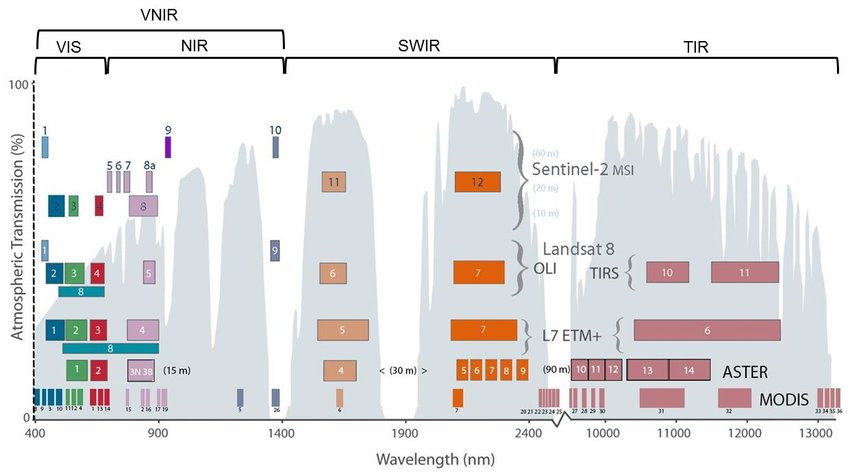
\includegraphics[width=1\linewidth]{common_optical_sensors_spectral_resolution} 

}

\caption{Common Optical Sensors and their Spectral Resolution}\label{fig:spectralres}
\end{figure}

There is an easy way to check the number of bands in Earth Engine, but no way to get an understanding of the relative \emph{spectral response} of the bands, where spectral response is a function measured in the laboratory to characterize the detector.

\begin{enumerate}
\def\labelenumi{\arabic{enumi}.}
\item
  To see the number of bands in an image, use:

\begin{Shaded}
\begin{Highlighting}[]
\CommentTok{// Get the MODIS band names as a List}
\KeywordTok{var}\NormalTok{ modisBands }\OperatorTok{=} \VariableTok{modisImage}\NormalTok{.}\AttributeTok{bandNames}\NormalTok{()}\OperatorTok{;}

\CommentTok{// Print the list.}
\AttributeTok{print}\NormalTok{(}\StringTok{'MODIS bands:'}\OperatorTok{,}\NormalTok{ modisBands)}\OperatorTok{;}

\CommentTok{// Print the length of the list.}
\AttributeTok{print}\NormalTok{(}\StringTok{'Length of the bands list:'}\OperatorTok{,} \VariableTok{modisBands}\NormalTok{.}\AttributeTok{length}\NormalTok{())}\OperatorTok{;}
\end{Highlighting}
\end{Shaded}
\item
  Note that only some of those bands contain radiometric data. Lots of them have other information, like quality control data. So the band listing isn't necessarily an indicator of spectral resolution, but can inform your investigation of the spectral resolution of the dataset. Try printing the bands from some of the other sensors to get a sense of spectral resolution.
\end{enumerate}

\begin{center}\rule{0.5\linewidth}{0.5pt}\end{center}

\textbf{Question 3.1: What is the spectral resolution of the MODIS instrument, and how did you determine it?}

\begin{center}\rule{0.5\linewidth}{0.5pt}\end{center}

\textbf{Question 3.2: Investigate the bands available for the USDA NASS Cropland Data Layers (CDL). What does the band information for the CDL represent? Which band(s) would you select if you were interested in evaluating the extent of pasture areas in the US? }

\begin{center}\rule{0.5\linewidth}{0.5pt}\end{center}

\hypertarget{temporal-resolution}{%
\subsection{Temporal Resolution}\label{temporal-resolution}}

Temporal resolution refers to the \emph{revisit time}, or temporal \emph{cadence} of a particular sensor's image stream. Think of this as the frequency of pixels in a time series at a given location.

\hypertarget{modis-1}{%
\subsubsection{MODIS}\label{modis-1}}

MODIS (either Terra or Aqua) produces imagery at approximately a daily cadence. To see the time series of images at a location, you can \texttt{print()} the \texttt{ImageCollection}, filtered to your area and date range of interest. For example, to see the MODIS images in 2011:

\begin{Shaded}
\begin{Highlighting}[]
\CommentTok{// Filter the MODIS mosaics to one year.   }
\KeywordTok{var}\NormalTok{ modisSeries }\OperatorTok{=} \VariableTok{myd09}\NormalTok{.}\AttributeTok{filterDate}\NormalTok{(}\StringTok{'2011-01-01'}\OperatorTok{,} \StringTok{'2011-12-31'}\NormalTok{)}\OperatorTok{;}      

\CommentTok{// Print the filtered  MODIS ImageCollection.   }
\AttributeTok{print}\NormalTok{(}\StringTok{'MODIS series:'}\OperatorTok{,}\NormalTok{ modisSeries)}\OperatorTok{;}  
\end{Highlighting}
\end{Shaded}

Expand the \texttt{features} property of the printed \texttt{ImageCollection} to see a \texttt{List} of all the images in the collection. Observe that the date of each image is part of the filename. Note the daily cadence. Observe that each MODIS image is a global mosaic, so there's no need to filter by location.

\hypertarget{landsat}{%
\subsubsection{Landsat}\label{landsat}}

Landsats (5 and later) produce imagery at 16-day cadence. TM and MSS are on the same satellite (Landsat 5), so it suffices to print the TM series to see the temporal resolution. Unlike MODIS, data from these sensors is produced on a scene basis, so to see a time series, it's necessary to filter by location in addition to time:

\begin{Shaded}
\begin{Highlighting}[]

   \CommentTok{// Filter to get a year's worth of TM scenes.}
  \KeywordTok{var}\NormalTok{ tmSeries }\OperatorTok{=}\NormalTok{ tm}
\NormalTok{  .}\AttributeTok{filterBounds}\NormalTok{(}\VariableTok{Map}\NormalTok{.}\AttributeTok{getCenter}\NormalTok{())}
\NormalTok{  .}\AttributeTok{filterDate}\NormalTok{(}\StringTok{'2011-01-01'}\OperatorTok{,} \StringTok{'2011-12-31'}\NormalTok{)}\OperatorTok{;}
  
  \CommentTok{// Print the filtered TM ImageCollection. }
  \AttributeTok{print}\NormalTok{(}\StringTok{'TM series:'}\OperatorTok{,}\NormalTok{ tmSeries)}\OperatorTok{;}
  
\end{Highlighting}
\end{Shaded}

\begin{enumerate}
\def\labelenumi{\arabic{enumi}.}
\item
  Again expand the \texttt{features} property of the printed \texttt{ImageCollection}. Note that a \href{http://landsat.usgs.gov/naming_conventions_scene_identifiers.php}{careful parsing of the TM image IDs} indicates the day of year (DOY) on which the image was collected. A slightly more cumbersome method involves expanding each Image in the list, expanding its properties and looking for the `DATE\_ACQUIRED' property.
\item
  To make this into a nicer list of dates, \href{https://en.wikipedia.org/wiki/Map_(higher-order_function)}{map()} a function over the ImageCollection. First define a function to get a Date from the metadata of each image, using the system properties:

\begin{Shaded}
\begin{Highlighting}[]
\KeywordTok{var}\NormalTok{ getDate }\OperatorTok{=} \KeywordTok{function}\NormalTok{(image) }\OperatorTok{\{}
\CommentTok{// Note that you need to cast the argument}
\KeywordTok{var}\NormalTok{ time }\OperatorTok{=} \VariableTok{ee}\NormalTok{.}\AttributeTok{Image}\NormalTok{(image).}\AttributeTok{get}\NormalTok{(}\StringTok{'system:time_start'}\NormalTok{)}\OperatorTok{;}
\CommentTok{// Return the time (in milliseconds since Jan 1, 1970) as a Date}
\ControlFlowTok{return} \VariableTok{ee}\NormalTok{.}\AttributeTok{Date}\NormalTok{(time)}\OperatorTok{;}
\OperatorTok{\};}
\end{Highlighting}
\end{Shaded}
\item
  Turn the \texttt{ImageCollection} into a \texttt{List} and\href{https://developers.google.com/earth-engine/getstarted\#mapping-what-to-do-instead-of-a-for-loop}{map() the function} over it:

\begin{Shaded}
\begin{Highlighting}[]
\KeywordTok{var}\NormalTok{ dates }\OperatorTok{=} \VariableTok{tmSeries}\NormalTok{.}\AttributeTok{toList}\NormalTok{(}\DecValTok{100}\NormalTok{).}\AttributeTok{map}\NormalTok{(getDate)}\OperatorTok{;}
\end{Highlighting}
\end{Shaded}
\item
  Print the result:

\begin{Shaded}
\begin{Highlighting}[]
\AttributeTok{print}\NormalTok{(dates)}\OperatorTok{;}
\end{Highlighting}
\end{Shaded}
\end{enumerate}

\begin{center}\rule{0.5\linewidth}{0.5pt}\end{center}

\textbf{Question 4 What is the temporal resolution of the Sentinel-2 satellites? How can you determine this from within GEE? }

\begin{center}\rule{0.5\linewidth}{0.5pt}\end{center}

\hypertarget{radiometric-resolution}{%
\subsection{Radiometric Resolution}\label{radiometric-resolution}}

Radiometric resolution refers to the ability of an imaging system to record many levels of brightness: \emph{coarse} radiometric resolution would record a scene with only a few brightness levels, whereas \emph{fine} radiometric resolution would record the same scene using many levels of brightness. Some also consider radiometric resolution to refer to the \emph{precision} of the sensing, or the level of \emph{quantization}.

Radiometric resolution is determined from the minimum radiance to which the detector is sensitive (Lmin), the maximum radiance at which the sensor saturates (Lmax), and the number of bits used to store the DNs (Q):

\[  \text{Radiometric resolution} = \frac{(L_{max} - L_{min})}{2^Q} \]

It might be possible to dig around in the metadata to find values for Lmin and Lmax, but computing radiometric resolution is generally not necessary unless you're studying phenomena that are distinguished by very subtle changes in radiance.

\hypertarget{resampling-and-reprojection}{%
\subsection{Resampling and ReProjection}\label{resampling-and-reprojection}}

Earth Engine makes every effort to handle projection and scale so that you don't have to. However, there are occasions where an understanding of projections is important to get the output you need. As an example, it's time to demystify the \href{https://developers.google.com/earth-engine/apidocs/ee-image-reproject}{reproject()} calls in the previous examples. Earth Engine requests inputs to your computations in the projection and scale of the output. The map attached to the playground has a \href{http://epsg.io/3857}{Maps Mercator projection}.

The scale is determined from the map's zoom level. When you add something to this map, Earth Engine secretly reprojects the input data to Mercator, resampling (with nearest neighbor) to screen resolution pixels based on the map's zoom level, then does all the computations with the reprojected, resampled imagery. In the previous examples, the reproject() calls force the computations to be done at the resolution of the input pixels: 1 meter.

\begin{enumerate}
\def\labelenumi{\arabic{enumi}.}
\item
  Re-run the edge detection code with and without the reprojection (Comment out all previous \texttt{Map.addLayer()} calls except for the original one)

\begin{Shaded}
\begin{Highlighting}[]
\CommentTok{// Zoom all the way in.}
\VariableTok{Map}\NormalTok{.}\AttributeTok{centerObject}\NormalTok{(point}\OperatorTok{,} \DecValTok{21}\NormalTok{)}\OperatorTok{;}
\CommentTok{// Display edges computed on a reprojected image.}
\VariableTok{Map}\NormalTok{.}\AttributeTok{addLayer}\NormalTok{(}\VariableTok{image}\NormalTok{.}\AttributeTok{convolve}\NormalTok{(laplacianKernel)}\OperatorTok{,} \OperatorTok{\{}\DataTypeTok{min}\OperatorTok{:} \DecValTok{0}\OperatorTok{,} \DataTypeTok{max}\OperatorTok{:} \DecValTok{255}\OperatorTok{\},} 
       \StringTok{'Edges with little screen pixels'}\NormalTok{)}\OperatorTok{;}
\CommentTok{// Display edges computed on the image at native resolution.}
\VariableTok{Map}\NormalTok{.}\AttributeTok{addLayer}\NormalTok{(edges}\OperatorTok{,} \OperatorTok{\{}\DataTypeTok{min}\OperatorTok{:} \DecValTok{0}\OperatorTok{,} \DataTypeTok{max}\OperatorTok{:} \DecValTok{255}\OperatorTok{\},} 
       \StringTok{'Edges with 1 meter pixels'}\NormalTok{)}\OperatorTok{;} 
\end{Highlighting}
\end{Shaded}

  What's happening here is that the projection specified in \texttt{reproject()} propagates backwards to the input, forcing all the computations to be performed in that projection. If you don't specify, the computations are performed in the projection and scale of the map (Mercator) at screen resolution.
\item
  You can control how Earth Engine resamples the input with \href{https://developers.google.com/earth-engine/guides/resample}{\texttt{resample()}}. By default, all resampling is done with the nearest neighbor. To change that, call \texttt{resample()} on the \emph{inputs}. Compare the input image, resampled to screen resolution with a bilinear and bicubic resampling:

\begin{Shaded}
\begin{Highlighting}[]
\CommentTok{// Resample the image with bilinear instead of the nearest neighbor.}
\KeywordTok{var}\NormalTok{ bilinearResampled }\OperatorTok{=} \VariableTok{image}\NormalTok{.}\AttributeTok{resample}\NormalTok{(}\StringTok{'bilinear'}\NormalTok{)}\OperatorTok{;}
\VariableTok{Map}\NormalTok{.}\AttributeTok{addLayer}\NormalTok{(bilinearResampled}\OperatorTok{,} \OperatorTok{\{\},} \StringTok{'input image, bilinear resampling'}\NormalTok{)}\OperatorTok{;}

\CommentTok{// Resample the image with bicubic instead of the nearest neighbor.}
\KeywordTok{var}\NormalTok{ bicubicResampled }\OperatorTok{=} \VariableTok{image}\NormalTok{.}\AttributeTok{resample}\NormalTok{(}\StringTok{'bicubic'}\NormalTok{)}\OperatorTok{;}
\VariableTok{Map}\NormalTok{.}\AttributeTok{addLayer}\NormalTok{(bicubicResampled}\OperatorTok{,} \OperatorTok{\{\},} \StringTok{'input image, bicubic resampling'}\NormalTok{)}\OperatorTok{;}
\end{Highlighting}
\end{Shaded}
\item
  Try zooming in and out, comparing to the input image resampled with the nearest with nearest neighbor (i.e.~without \texttt{resample()} called on it).

  \textbf{You should rarely, if ever, have to use \texttt{reproject()} and \texttt{resample()}.} Do not use \texttt{reproject()} or \texttt{resample()} unless necessary. They are only used here for demonstration purposes.
\end{enumerate}

\hypertarget{additional-exercises}{%
\subsection{Additional Exercises}\label{additional-exercises}}

Now that we have some familiarity with higher quality images, lets look at a few from the (broken) Landsat 7 satellite. Using your downloading skills, now select an image that contains the Blacksburg area with minimal cloud cover from Landsat 7 (for now, using the Collection 1 Tier 1 calibrated top-of-atmosphere (TOA) reflectance data product). Look at the image.

\textbf{Question 5: What is the obvious (hint: post-2003) problem with the Landsat 7 image? What is the nature of that problem and what have some researchers done to try to correct it?} (please research online in addition to using what you have learned in class/from the book)

\begin{center}\rule{0.5\linewidth}{0.5pt}\end{center}

\textbf{Question 6: Name three major changes you can view in the Blacksburg Area in the last decade using any of the above imagery (and state the source).}

\begin{center}\rule{0.5\linewidth}{0.5pt}\end{center}

Conduct a search to compare the technical characteristics of the following sensors:

\begin{enumerate}
\def\labelenumi{(\roman{enumi})}
\tightlist
\item
  MODIS (NASA) versus Sentinel (ESA), and
\item
  AVHRR (NASA) versus IRS-P6 (or choose another Indian Remote Sensing satellite)
\end{enumerate}

\textbf{Question 7: Based on the characteristics you describe, for which applications is one sensor likely to be more suitable than the other ones? }

Note: when using the internet to answer this question, be sure to cite your sources and ensure that you are obtaining information from an official, reputable source!

\begin{center}\rule{0.5\linewidth}{0.5pt}\end{center}

\hypertarget{where-to-submit}{%
\subsection*{Where to submit}\label{where-to-submit}}
\addcontentsline{toc}{subsection}{Where to submit}

Submit your responses to these questions on \href{https://www.gradescope.com/courses/293173/assignments/1446622/submissions}{Gradescope} by 10am on Wednesday, September 8. All students who have been attending class have already been enrolled in Gradescope, although if for some reason you need to sign up again, the access code for our course is \texttt{6PEW3W}.

\end{document}
